%iffalse
\let\negmedspace\undefined
\let\negthickspace\undefined
\documentclass[journal,12pt,onecolumn]{IEEEtran}
\usepackage{cite}
\usepackage{amsmath,amssymb,amsfonts,amsthm}
\usepackage{algorithmic}
\usepackage{graphicx}
\usepackage{textcomp}
\usepackage{xcolor}
\usepackage{txfonts}
\usepackage{listings}
\usepackage{enumitem}
\usepackage{mathtools}
\usepackage{gensymb}
\usepackage{comment}
\usepackage[breaklinks=true]{hyperref}
\usepackage{tkz-euclide} 
\usepackage{listings}
\usepackage{gvv}                                        
%\def\inputGnumericTable{}                                 
\usepackage[latin1]{inputenc}     
\usepackage{xparse}
\usepackage{color}                                            
\usepackage{array}                                            
\usepackage{longtable}                                       
\usepackage{calc}                                             
\usepackage{multirow}
\usepackage{multicol}
\usepackage{hhline}                                           
\usepackage{ifthen}                                           
\usepackage{lscape}
\usepackage{tabularx}
\usepackage{array}
\usepackage{float}
\newtheorem{theorem}{Theorem}[section]
\newtheorem{problem}{Problem}
\newtheorem{proposition}{Proposition}[section]
\newtheorem{lemma}{Lemma}[section]
\newtheorem{corollary}[theorem]{Corollary}
\newtheorem{example}{Example}[section]
\newtheorem{definition}[problem]{Definition}
\newcommand{\BEQA}{\begin{eqnarray}}
\newcommand{\EEQA}{\end{eqnarray}}
\usepackage{float}
%\newcommand{\define}{\stackrel{\triangle}{=}}
\theoremstyle{remark}
\usepackage{ circuitikz }
%\newtheorem{rem}{Remark}
% Marks the beginning of the document


\title{GATE-IN-2016}
\author{EE25BTECH11002 - Achat Parth Kalpesh }
\date{}

\begin{document}

\maketitle
\section*{Q.1-Q.5 carry one mark each. }

\begin{enumerate}
\item An apple costs Rs. $10$. An onion costs Rs. $8$.
Select the most suitable sentence with respect to grammar and usage.

\hfill{(GATE IN 2016)}
\begin{enumerate}

\item The price of an apple is greater than an onion.
\item The price of an apple is more than onion.
\item The price of an apple is greater than that of an onion.
\item Apples are more costlier than onions.

\end{enumerate}

\item The Buddha said, "Holding on to anger is like \underline{grasping} a hot coal with the intent of throwing it at someone else; you are the one who gets burnt."
Select the word below which is closest in meaning to the word underlined above.

\hfill{(GATE IN 2016)}
\begin{enumerate}
\begin{multicols}{4}
\item burning
\item igniting
\item clutching
\item flinging
\end{multicols}
\end{enumerate}

\item M has a son Q and a daughter R. He has no other children. E is the mother of P and daughter-in-law of M. How is P related to M?

\hfill{(GATE IN 2016)}
\begin{enumerate}
\begin{multicols}{2}
\item P is the son-in-law of M.
\item P is the grandchild of M.
\item P is the daughter-in law of M.
\item P is the grandfather of M.
\end{multicols}
\end{enumerate}

\item The number that least fits this set: \brak{\text{324, 441, 97 and 64}} is \rule{2cm}{0.4pt}.

\hfill{(GATE IN 2016)}
\begin{enumerate}
\begin{multicols}{4}
\item 324
\item 441
\item 97
\item 64
\end{multicols}
\end{enumerate}

\item It takes $10$ s and $15$ s, respectively, for two trains travelling at different constant speeds to completely pass a telegraph post. The length of the first train is $120$ m and that of the second train is $150$ m. The magnitude of the difference in the speeds of the two trains \brak{\text{in m/s}} is \rule{2cm}{0.4pt}.

\hfill{(GATE IN 2016)}
\begin{enumerate}
\begin{multicols}{4}
\item 2.0
\item 10.0
\item 12.0
\item 22.0
\end{multicols}
\end{enumerate}

\textbf{Q.6 - Q.10 carry two marks each.}

\item The velocity V of a vehicle along a straight line is measured in m/s and plotted as shown\figref{fig:z1} with respect to time in seconds. At the end of the $7$ seconds, how much will the odometer reading increase by \brak{\text{in m}}?

\begin{figure}[H]
\centering
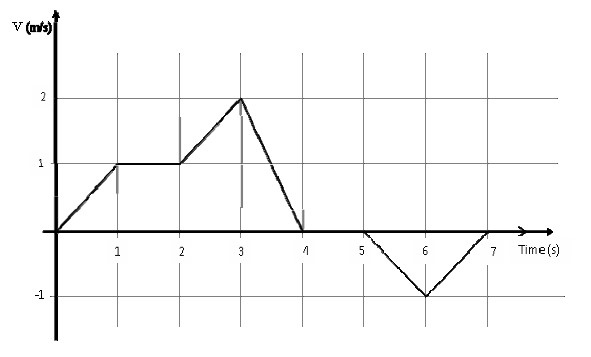
\includegraphics[width=0.8\columnwidth]{figs/z1.jpg}
\caption*{}
\label{fig:z1}
\end{figure}



\hfill{(GATE IN 2016)}
\begin{enumerate}
\begin{multicols}{4}
\item 0
\item 3
\item 4
\item 5
\end{multicols}
\end{enumerate}

\item The overwhelming number of people infected with rabies in India has been flagged by the World Health Organization as a source of concern. It is estimated that inoculating $70\%$ of pets and stray dogs against rabies can lead to a significant reduction in the number of people infected with rabies.
Which of the following can be logically inferred from the above sentences?

\hfill{(GATE IN 2016)}
\begin{enumerate}
\item The number of people in India infected with rabies is high.
\item The number of people in other parts of the world who are infected with rabies is low.
\item Rabies can be eradicated in India by vaccinating $70\%$ of stray dogs.
\item Stray dogs are the main source of rabies worldwide.
\end{enumerate}

\item A flat is shared by four first year undergraduate students. They agreed to allow the oldest of them to enjoy some extra space in the flat. Manu is two months older than Sravan, who is three months younger than Trideep. Pavan is one month older than Sravan. Who should occupy the extra space in the flat?

\hfill{(GATE IN 2016)}
\begin{enumerate}
\begin{multicols}{4}
\item Manu
\item Sravan
\item Trideep
\item Pavan
\end{multicols}
\end{enumerate}

\item Find the area bounded by the lines $3x+2y=14$, $2x-3y=5$ in the first quadrant.

\hfill{(GATE IN 2016)}
\begin{enumerate}
\begin{multicols}{4}
\item 14.95
\item 15.25
\item 15.70
\item 20.35
\end{multicols}
\end{enumerate}

\item A straight line is fit to a data set \brak{\ln x, y}. This line intercepts the abscissa at $\ln x = 0.1$ and has a slope of $-0.02$. What is the value of y at $x = 5$ from the fit?

\hfill{(GATE IN 2016)}
\begin{enumerate}
\begin{multicols}{4}
\item -0.030
\item -0.014
\item 0.014
\item 0.030
\end{multicols}
\end{enumerate}

\end{enumerate}

\section*{END OF THE QUESTION PAPER }


\textbf{Q. 1 - Q. 25 carry one mark each}

\begin{enumerate}
\item A straight line of the form $y = mx + c$ passes through the origin and the point \brak{x, y} = \brak{2, 6}. The value of m is \rule{2cm}{0.4pt}.

\hfill{(GATE IN 2016)}

\item $\lim_{n \to \infty} \brak{\sqrt{n^2+n} - \sqrt{n^2+1}}$ is \rule{2cm}{0.4pt}.

\hfill{(GATE IN 2016)}

\item A voltage $V_1$ is measured $100$ times and its average and standard deviation are $100$ V and $1.5$ V respectively. A second voltage $V_2$, which is independent of $V_1$, is measured $200$ times and its average and standard deviation are $150$ V and $2$ V respectively. $V_3$ is computed as: $V_3 = V_1 + V_2$. Then the standard deviation of $V_3$ in volt is \rule{2cm}{0.4pt}.

\hfill{(GATE IN 2016)}

\item The vector that is NOT perpendicular to the vectors \brak{i + j + k} and \brak{i + 2j + 3k} is \rule{2cm}{0.4pt}.

\hfill{(GATE IN 2016)}
\begin{enumerate}
\begin{multicols}{4}
\item \brak{i-2j+k}
\item \brak{-i + 2j-k}
\item \brak{0i + 0j + 0k}
\item \brak{4i +3 j + 5k}
\end{multicols}
\end{enumerate}

\item In the neighborhood of $z = 1$, the function $f\brak{z}$ has a power series expansion of the form 
\begin{align*}
f\brak{z} = 1 + \brak{1 - z} + \brak{1 - z}^2 + \dots\dots\dots\dots\dots
\end{align*}
Then $f\brak{z}$ is

\hfill{(GATE IN 2016)}
\begin{enumerate}
\begin{multicols}{2}
\item $\frac{1}{z}$
\item $\frac{-1}{z-2}$
\item $\frac{z-1}{z+1}$
\item $\frac{1}{2z-1}$
\end{multicols}
\end{enumerate}

\item Three currents $i_1, i_2$ and $i_3$ meet at a node as shown in the figure below.\figref{fig:z2} If $i_1 = 3 \cos\brak{\omega t}$ ampere, $i_2 = 4 \sin\brak{\omega t}$ ampere and $i_3 = I_3 \cos\brak{\omega t + \theta}$ ampere, the value of $I_3$ in ampere is \rule{2cm}{0.4pt}.

\begin{figure}[h!]
\centering
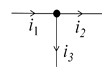
\includegraphics[width=0.2\columnwidth]{figs/z2.jpg}
\caption*{}
\label{fig:z2}
\end{figure}


\hfill{(GATE IN 2016)}

\item An air cored coil has a Q of $5$ at a frequency of $100$ kHz. The Q of the coil at $20$ kHz \brak{\text{neglecting skin effect}} will be \rule{2cm}{0.4pt}.

\hfill{(GATE IN 2016)}

\item A current $i\brak{t}$ shown in the figure below\figref{fig:z3} is passed through a $1$ F capacitor that had zero initial charge. The voltage across the capacitor for $t > 2$ s in volt is \rule{2cm}{0.4pt}.

\begin{figure}[H]
\centering
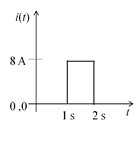
\includegraphics[width=0.4\columnwidth]{figs/z3.jpg}
\caption*{}
\label{fig:z3}
\end{figure}

\hfill{(GATE IN 2016)}

\item The signal $x\sbrak{n}$ shown in the figure below\figref{fig:z4} is convolved with itself to get $y\sbrak{n}$. The value of $y\sbrak{-1}$ is \rule{2cm}{0.4pt}.

\begin{figure}[H]
\centering
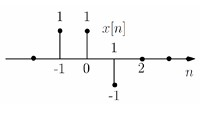
\includegraphics[width=0.5\columnwidth]{figs/z4.jpg}
\caption*{}
\label{fig:z4}
\end{figure}

\hfill{(GATE IN 2016)}

\item In the circuit shown below\figref{fig:z5} $\brak{v_1 + v_2} = \sbrak{1 \sin\brak{2\pi 10000t} + 1 \sin\brak{2\pi 30000t}}$ V. The RMS value of the current through the resistor R will be minimum if the value of the capacitor C in microfarad is \rule{2cm}{0.4pt}.

\begin{figure}[H]
\centering
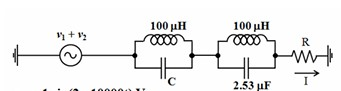
\includegraphics[width=0.8\columnwidth]{figs/z5.jpg}
\caption*{}
\label{fig:z5}
\end{figure}

\hfill{(GATE IN 2016)}

\item If $X\brak{s}$, the Laplace transform of signal $x\brak{t}$ is given by $X\brak{s} = \frac{\brak{s+2}}{\brak{s+1}\brak{s+3}^2}$, then the value of $x\brak{t}$ as $t \to \infty$ is \rule{2cm}{0.4pt}.

\hfill{(GATE IN 2016)}

\item The number of times the Nyquist plot of $G\brak{s} = \frac{s-1}{s+1}$ will encircle the origin clockwise is \rule{2cm}{0.4pt}.

\hfill{(GATE IN 2016)}

\item The value of $a_o$ which will ensure that the polynomial $s^3 + 3s^2 + 2s + a_o$ has roots on the left half of the s-plane is

\hfill{(GATE IN 2016)}
\begin{enumerate}
\begin{multicols}{4}
\item 11
\item 9
\item 7
\item 5
\end{multicols}
\end{enumerate}

\item The input $i\brak{t} = 2\sin\brak{3t + \pi}$ is applied to a system whose transfer function $G\brak{s} = \frac{8}{\brak{s+10}^2}$.
The amplitude of the output of the system is \rule{2cm}{0.4pt}.

\hfill{(GATE IN 2016)}

\item The diode D used in the circuit below\figref{fig:z6} is ideal. The voltage drop $V_{ab}$ across the $1$ k$\ohm$ resistor in volt is \rule{2cm}{0.4pt}.
\begin{figure}[H]
\centering
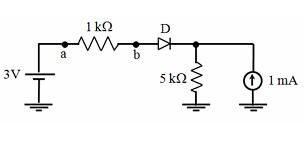
\includegraphics[width=0.6\columnwidth]{figs/z6.jpg}
\caption*{}
\label{fig:z6}
\end{figure}

\hfill{(GATE IN 2016)}

\item In the circuit given below,\figref{fig:z7} the opamp is ideal. The output voltage $V_O$ in volt is \rule{2cm}{0.4pt}.
\begin{figure}[H]
\centering
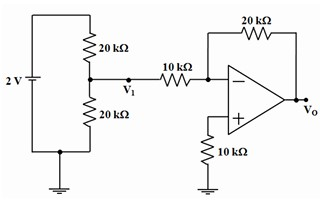
\includegraphics[width=0.5\columnwidth]{figs/z7.jpg}
\caption*{}
\label{fig:z7}
\end{figure}

\hfill{(GATE IN 2016)}

\item In the circuit given below,\figref{fig:z8} the diodes $D_1$ and $D_2$ have a forward voltage drop of $0.6$ V. The opamp used is ideal. The magnitude of the negative peak value of the output $V_O$ in volt is \rule{2cm}{0.4pt}.
\begin{figure}[H]
\centering
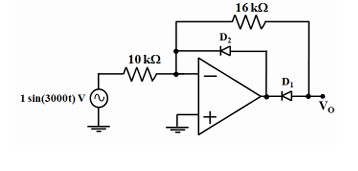
\includegraphics[width=0.6\columnwidth]{figs/z8.jpg}
\caption*{}
\label{fig:z8}
\end{figure}

\hfill{(GATE IN 2016)}

\item The Boolean expression $XY + \brak{ X'+ Y' }Z$ is equivalent to

\hfill{(GATE IN 2016)}
\begin{enumerate}
\begin{multicols}{4}
\item $XYZ' + X'Y'Z$
\item $X'Y'Z' + XYZ$
\item $\brak{ X + Z }\brak{Y+Z}$
\item $\brak{ X' + Z }\brak{ Y' + Z }$
\end{multicols}
\end{enumerate}

\item In the digital circuit given below,\figref{fig:z9} F is
\begin{figure}[H]
\centering
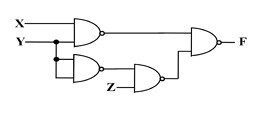
\includegraphics[width=0.4\columnwidth]{figs/z9.jpg}
\caption*{}
\label{fig:z9}
\end{figure}

\hfill{(GATE IN 2016)}
\begin{enumerate}
\begin{multicols}{4}
\item $XY + Y\bar{Z}$
\item $XY + \bar{Y}Z$
\item $\bar{X}Y + YZ$
\item $XZ + \bar{Y}$
\end{multicols}
\end{enumerate}

\item A $3\frac{1}{2}$ digit DMM has an accuracy specification of $\pm 1\%$ of full scale \brak{\text{accuracy class 1}}. A reading of $100.0$ mA is obtained on its $200$ mA full scale range. The worst case error in the reading in milliampere is \rule{2cm}{0.4pt}.

\hfill{(GATE IN 2016)}

\item  A dc potentiometer, shown in figure below,\figref{fig:z10} is made by connecting fifteen 10 $\ohm$ resistors and a 10 $\ohm$ slide wire of length 1000 mm in series. The potentiometer is standardized with the current $I_p = 10.0000$ mA. Balance for an unknown voltage is obtained when the dial is in position 11 \brak{\text{11 numbers of the fixed 10 $\ohm$ resistor are included}} and the slide wire is on the $234$th mm position. The unknown voltage \brak{\text{up to four decimal places}} in volt is \rule{2cm}{0.4pt}.

\begin{figure}[H]
\centering
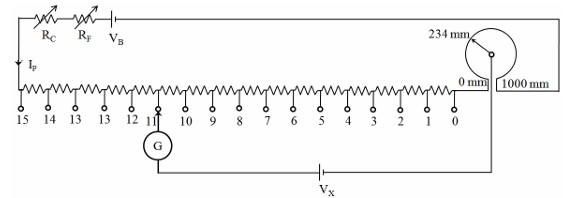
\includegraphics[width=1\columnwidth]{figs/z10.jpg}
\caption*{}
\label{fig:z10}
\end{figure}

\hfill{(GATE IN 2016)}

\item In the circuit given below,\figref{fig:z11} each input terminal of the opamp draws a bias current of $10$ nA. The effect due to these input bias currents on the output voltage $V_O$ will be zero, if the value of R chosen in kilo-ohm is \rule{2cm}{0.4pt}.
\begin{figure}[H]
\centering
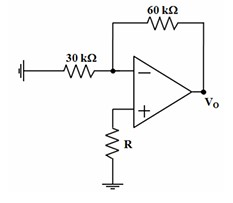
\includegraphics[width=0.4\columnwidth]{figs/z11.jpg}
\caption*{}
\label{fig:z11}
\end{figure}
\hfill{(GATE IN 2016)}

\item A peizo-electric type pressure sensor has a sensitivity of $1$ mV/kPa and a bandwidth of $300$ Hz to $300$ kHz. For a constant \brak{dc} pressure of $100$ kPa, the steady state output of the sensor in millivolt is \rule{2cm}{0.4pt}.

\hfill{(GATE IN 2016)}

\item The signal $m\brak{t} = \cos\brak{\omega_m t}$ is SSB \brak{\text{single side-band}} modulated with a carrier $\cos\brak{\omega_c t}$ to get $s\brak{t}$. The signal obtained by passing $s\brak{t}$ through an ideal envelope detector is

\hfill{(GATE IN 2016)}
\begin{enumerate}
\begin{multicols}{4}
\item $\cos\brak{\omega_m t}$
\item $\sin\brak{\omega_m t}$
\item $\cos\brak{\omega_m t} + \sin\brak{\omega_m t}$
\item 1
\end{multicols}
\end{enumerate}

\item Let $s\brak{t} = \text{rect}\brak{\frac{t-3}{3}}$ be a signal passed through an AWGN \brak{\text{additive white Gaussian noise}} channel with noise power spectral density \brak{PSD} $\frac{N_0}{2}$ to get $v\brak{t}$. If $v\brak{t}$ is passed through a matched-filter that is matched to $s\brak{t}$, then output signal-to noise ratio \brak{SNR} of the matched-filter is

\hfill{(GATE IN 2016)}
\begin{enumerate}
\begin{multicols}{4}
\item $\frac{1}{N_0}$
\item $\frac{2}{N_0}$
\item $\frac{3}{N_0}$
\item $\frac{4}{N_0}$
\end{multicols}
\end{enumerate}

\textbf{Q. 26 - Q. 55 carry two marks each. }

\item Let $f: \sbrak{-1,1}\to \mathbb{R}$, where $f\brak{x} = 2x^3 - x^4 - 10$. The minimum value of $f\brak{x}$ is \rule{2cm}{0.4pt}.

\hfill{(GATE IN 2016)}

\item An urn contains $5$ red and $7$ green balls. A ball is drawn at random and its colour is noted. The ball is placed back into the urn along with another ball of the same colour. The probability of getting a red ball in the next draw is

\hfill{(GATE IN 2016)}
\begin{enumerate}
\begin{multicols}{4}
\item $\frac{65}{156}$
\item $\frac{67}{156}$
\item $\frac{79}{156}$
\item $\frac{89}{156}$
\end{multicols}
\end{enumerate}

\item Consider the matrix

\begin{align}
A = \myvec{2 & 1 & 1 \\ 2 & 3 & 4 \\ -1 & -1 & -2}
\end{align}

whose eigenvalues are $1, -1$ and $3$. Then Trace of $\brak{A^3 - 3A^2}$ is \rule{2cm}{0.4pt}.

\hfill{(GATE IN 2016)}

\item The relationship between the force $f\brak{t}$ and the displacement $x\brak{t}$ of a spring-mass system \\ \brak{\text{with a mass M, viscous damping D and spring constant K}} is
\begin{align}
M\frac{d^2x\brak{t}}{dt^2} + D \frac{d x\brak{t}}{dt}\brak{t}+Kx\brak{t} = f\brak{t}.
\end{align}

$X\brak{s}$ and $F\brak{s}$ are the Laplace transforms of $x\brak{t}$ and $f\brak{t}$ respectively. With $M = 0.1, D = 2, K = 10$ in appropriate units, the transfer function $G\brak{s} = \frac{X\brak{s}}{F\brak{s}}$ is

\hfill{(GATE IN 2016)}
\begin{enumerate}
\begin{multicols}{2}
\item $\frac{10}{s^2 + 20s + 100}$
\item $s^2 + 20s + 100$
\item $\frac{10s^2}{s^2 + 20s + 100}$
\item $\frac{s}{s^2 + 20s + 100}$
\end{multicols}
\end{enumerate}

\item The value of the integral $\frac{1}{2\pi j} \oint_C \frac{z^2+1}{z^2-1} dz$ where z is a complex number and C is a unit circle with center at $1+0j$ in the complex plane is \rule{2cm}{0.4pt}.

\hfill{(GATE IN 2016)}

\item The current $I_x$ in the circuit given below\figref{fig:z12} in milliampere is \rule{2cm}{0.4pt}.
\begin{figure}[H]
\centering
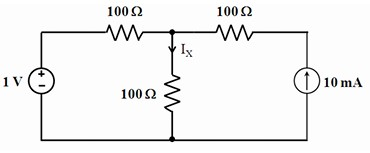
\includegraphics[width=0.6\columnwidth]{figs/z12.jpg}
\caption*{}
\label{fig:q12}
\end{figure}

\hfill{(GATE IN 2016)}

\item In the circuit shown below,\figref{fig:z13} $V_s = 101\angle 0$ V, $R = 10$ $\ohm$ and $\omega L= 100$ $\ohm$. The current $I_s$ is in phase with $V_s$. The magnitude of $I_s$ in milliampere is \rule{2cm}{0.4pt}.
\begin{figure}[H]
\centering
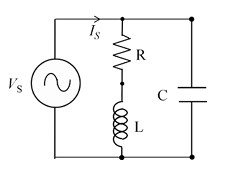
\includegraphics[width=0.4\columnwidth]{figs/z13.jpg}
\caption*{}
\label{fig:z13}
\end{figure}

\hfill{(GATE IN 2016)}

\item A symmetrical three-phase three-wire RYB system is connected to a balanced delta-connected load. The RMS values of the line current and line-to-line voltage are $10$ A and $400$ V respectively. The power in the system is measured using the two wattmeter method. The first wattmeter connected between R-line and Y-line reads zero. The reading of the second wattmeter \brak{\text{connected between B-line and Y-line}} in watt is \rule{2cm}{0.4pt}.

\hfill{(GATE IN 2016)}

\item In the strain gauge bridge circuit given below,\figref{fig:z14} $R_1 = R_3 = R \brak{1 - x}$ and $R_2 = R_4 = R \brak{1 + x}$, where R is $350$ $\ohm$. The voltage sources $v_s$ and $v_n$ represent the dc excitation and the undesired noise/interference, respectively. The value of capacitor C in microfarad that is required to ensure that the output across a and b is low-pass filtered with a cutoff frequency of $150$ Hz is \rule{2cm}{0.4pt}.
\begin{figure}[H]
\centering
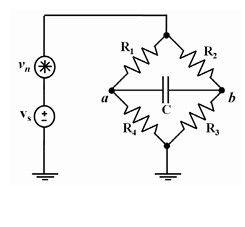
\includegraphics[width=0.5\columnwidth]{figs/z14.jpg}
\caption*{}
\label{fig:z14}
\end{figure}

\hfill{(GATE IN 2016)}

\item The voltage $v\brak{t}$ shown below\figref{fig:z15} is applied to the given circuit. $v\brak{t} = 3$ V for $t < 0$ and $v\brak{t} = 6$ V for $t > 0$. The value of current $i\brak{t}$ at $t = 1$s, in ampere is \rule{2cm}{0.4pt}.
\begin{figure}[H]
\centering
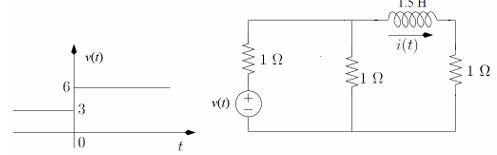
\includegraphics[width=1\columnwidth]{figs/z15.jpg}
\caption*{}
\label{fig:z15}
\end{figure}

\hfill{(GATE IN 2016)}

\item For the periodic signal $x\brak{t}$ shown below\figref{fig:z16} with period $T = 8$s, the power in the $10^{th}$ harmonic is
\begin{figure}[H]
\centering
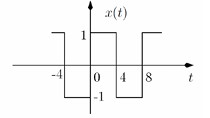
\includegraphics[width=0.5\columnwidth]{figs/z16.jpg}
\caption*{}
\label{fig:z16}
\end{figure}

\hfill{(GATE IN 2016)}
\begin{enumerate}
\begin{multicols}{4}
\item 0
\item $\frac{1}{2}\brak{\frac{2}{10\pi}}^2$
\item $\frac{1}{2}\brak{\frac{4}{10\pi}}^2$
\item $\frac{1}{2}\brak{\frac{4}{5\pi}}^2$
\end{multicols}
\end{enumerate}

\item The fundamental period $N_0$ of the discrete-time sinusoid $x\sbrak{n} = \sin\brak{\frac{301}{4}\pi n}$ is \rule{2cm}{0.4pt}.

\hfill{(GATE IN 2016)}

\item The transfer function G\brak{s} of a system which has the asymptotic Bode plot shown below\figref{fig:z17} is
\begin{figure}[H]
\centering
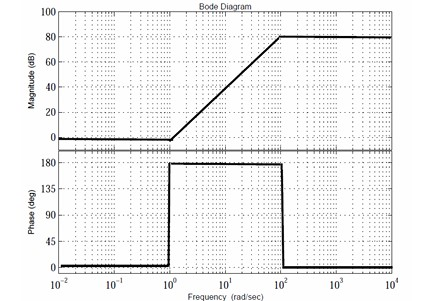
\includegraphics[width=1\columnwidth]{figs/z17.jpg}
\caption*{}
\label{fig:z17}
\end{figure}

\hfill{(GATE IN 2016)}
\begin{enumerate}
\begin{multicols}{2}
\item $10^4 \frac{\brak{s-1}^2}{\brak{s+100}^2}$
\item $10^4 \frac{\brak{s+1}^2}{\brak{s+100}^2}$
\item $10^4 \frac{\brak{s+1}}{\brak{s+100}^2}$
\item $10^4 \frac{\brak{s-1}^2}{\brak{s-100}^2}$
\end{multicols}
\end{enumerate}

\item For the feedback system given below,\figref{fig:z18} the transfer function $G\brak{s} = \frac{1}{\brak{s+1}^2}$. The system CANNOT be stabilized with
\begin{figure}[H]
\centering
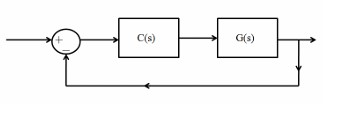
\includegraphics[width=0.6\columnwidth]{figs/z18.jpg}
\caption*{}
\label{fig:z18}
\end{figure}

\hfill{(GATE IN 2016)}
\begin{enumerate}
\begin{multicols}{2}
\item $C\brak{s}=1+\frac{3}{s}$
\item $C\brak{s} = 3+\frac{7}{s}$
\item $C\brak{s} = 3+\frac{9}{s}$
\item $C\brak{s} = \frac{1}{s}$
\end{multicols}
\end{enumerate}

\item Match the unit-step responses \brak{1}, \brak{2} and \brak{3} with the transfer functions P\brak{s}, Q\brak{s} and R\brak{s}, given below.\figref{fig:z19}

\begin{figure}[H]
\centering
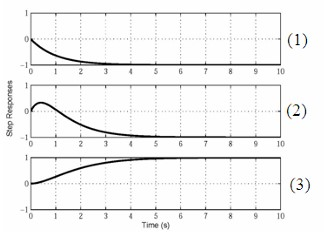
\includegraphics[width=0.7\columnwidth]{figs/z19.jpg}
\caption*{}
\label{fig:qz19}
\end{figure}


\begin{table}[h]
\centering
\begin{tabular}{|c|c|}
\hline
$P\brak{s}=$ & $\frac{-1}{\brak{s+1}}$ \\
\hline
$Q\brak{s}=$ & $\frac{2\brak{s-1}}{\brak{s+10}\brak{s+2}}$ \\
\hline
$R\brak{s}=$ & $\frac{1}{\brak{s+1}^2}$ \\
\hline
\end{tabular}
\caption*{}
\label{tab:q40}
\end{table}


\hfill{(GATE IN 2016)}
\begin{enumerate}
\begin{multicols}{2}
\item P\brak{s} - \brak{3}, Q\brak{s} - \brak{2}, R\brak{s} - \brak{1}
\item P\brak{s} - \brak{1}, Q\brak{s} - \brak{2}, R\brak{s} - \brak{3}
\item P\brak{s} - \brak{2}, Q\brak{s} - \brak{1}, R\brak{s} - \brak{3}
\item P\brak{s} - \brak{1}, Q\brak{s} - \brak{3}, R\brak{s} - \brak{2}
\end{multicols}
\end{enumerate}

\item An ideal opamp is used to realize a difference amplifier circuit given below\figref{fig:z20} having a gain of $10$. If $x = 0.025$, the CMRR of the circuit in dB is \rule{2cm}{0.4pt}.
\begin{figure}[H]
\centering
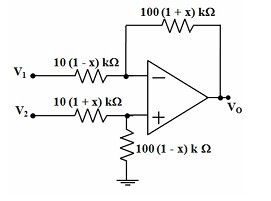
\includegraphics[width=0.5\columnwidth]{figs/z20.jpg}
\caption*{}
\label{fig:z20}
\end{figure}

\hfill{(GATE IN 2016)}

\item In the circuit given below,\figref{fig:z21} the opamp is ideal. The input $v_x$ is a sinusoid. To ensure $v_y = v_x$, the value of $C_N$ in picofarad is \rule{2cm}{0.4pt}.
\begin{figure}[H]
\centering
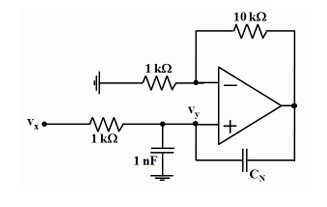
\includegraphics[width=0.5\columnwidth]{figs/z21.jpg}
\caption*{}
\label{fig:z21}
\end{figure}

\hfill{(GATE IN 2016)}

\item In the circuit given below,\figref{fig:z22} the opamp is ideal. The value of current $I_L$ in microampere is \rule{2cm}{0.4pt}.
\begin{figure}[H]
\centering
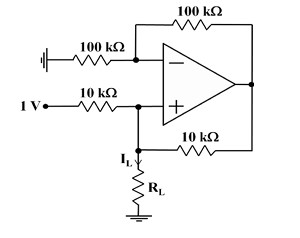
\includegraphics[width=0.5\columnwidth]{figs/z22.jpg}
\caption*{}
\label{fig:z22}
\end{figure}

\hfill{(GATE IN 2016)}

\item A 4 to 1 multiplexer to realize a Boolean function F \brak{X, Y, Z} is shown in the figure below.\figref{fig:z23} The inputs Y and Z are connected to the selectors of the MUX \brak{\text{Y is more significant}}. The canonical sum-of-product expression for F \brak{X, Y, Z} is
\begin{figure}[H]
\centering
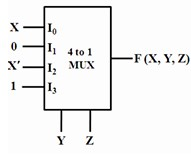
\includegraphics[width=0.4\columnwidth]{figs/z23.jpg}
\caption*{}
\label{fig:z23}
\end{figure}

\hfill{(GATE IN 2016)}
\begin{enumerate}
\begin{multicols}{2}
\item $\sum m \brak{ 2, 3, 4, 7 }$
\item $\sum m \brak{ 1, 3, 5, 7 }$
\item $\sum m \brak{ 0, 2, 4, 6}$
\item $\sum m \brak{ 2, 3, 5, 6 }$
\end{multicols}
\end{enumerate}

\item A synchronous counter using two J K flip flops that goes through the sequence of states: $Q_1 Q_2 = 00 \to 10 \to 01 \to 11 \to 00 \dots$ is required. To achieve this, the inputs to the flip flops are\figref{fig:z24}
\begin{figure}[H]
\centering
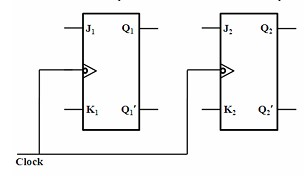
\includegraphics[width=0.6\columnwidth]{figs/z24.jpg}
\caption*{}
\label{fig:z24}
\end{figure}

\hfill{(GATE IN 2016)}
\begin{enumerate}
\begin{multicols}{2}
\item $J_1= Q_2, K_1 = 0; J_2= Q_1', K_2= Q_1$
\item $J_1= 1, K_1 = 1; J_2=Q_1, K_2=Q_1$
\item $J_1= Q_2, K_1 = Q_2'; J_2=1, K_2=1$
\item $J_1= Q_2', K_1= Q_2; J_2 = Q_1, K_2=Q_1'$
\end{multicols}
\end{enumerate}

\item A 1 Kbyte memory module has to be interfaced with an 8-bit microprocessor that has 16 address lines. The address lines $A_0$ to $A_9$ of the processor are connected to the corresponding address lines of the memory module. The active low chip select $\overline{CS}$ of the memory module is connected to the $y_5$ output of a 3 to 8 decoder with active low outputs. $S_0, S_1$, and $S_2$ are the input lines to the decoder, with $S_2$ as the MSB. The decoder has one active low $\overline{EN1}$ and one active high $EN_2$ enable lines as shown below.\figref{fig:z25} The address range\brak{s} that gets mapped onto this memory module is \brak{are}
\begin{figure}[H]
\centering
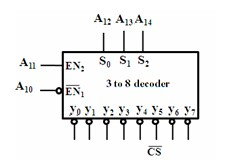
\includegraphics[width=0.6\columnwidth]{figs/z25.jpg}
\caption*{}
\label{fig:z25}
\end{figure}

\hfill{(GATE IN 2016)}
\begin{enumerate}

\item $3000_H$ to $33FF_H$ and $E000_H$ to $E3FF_H$
\item $1400_H$ to $17FF_H$
\item $5300_H$ to $53FF_H$ and $A300_H$ to $A3FF_H$
\item $5800_H$ to $5BFF_H$ and $D800_H$ to $DBFF_H$

\end{enumerate}

\item A coil is tested with a series type Q-meter. Resonance at a particular frequency is obtained with a capacitance of $110$ pF. When the frequency is doubled, the capacitance required for resonance is $20$ pF. The distributed capacitance of the coil in pico farad is \rule{2cm}{0.4pt}.

\hfill{(GATE IN 2016)}

\item The comparators \brak{\text{output = '1', when input $>$ 0 and output ='0', when input $<$ 0}}, exclusive-OR gate and the unity gain low-pass filter given in the circuit are ideal. The logic output voltages of the exclusive-OR gate are $0$ V and $5$ V. The cutoff frequency of the low-pass filter is $0.1$ Hz. For $V_1 = 1 \sin\brak{3000t + 36\degree}$ V and $V_2 = 1 \sin\brak{3000t}$ V, the value of $V_O$ in volt is \rule{2cm}{0.4pt}.\figref{fig:z26}
\begin{figure}[H]
\centering
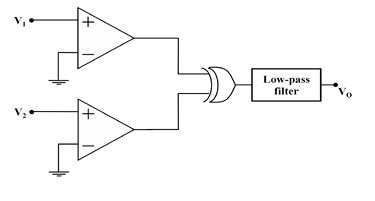
\includegraphics[width=0.8\columnwidth]{figs/z26.jpg}
\caption*{}
\label{fig:z26}
\end{figure}

\hfill{(GATE IN 2016)}

\item A $200$ mV full scale dual-slope $3\frac{1}{2}$ digit DMM has a reference voltage of $100$ mV and a first integration time of $100$ ms. For an input of $\sbrak{100 + 10 \cos\brak{100\pi t}}$ mV, the conversion time \brak{without taking the auto-zero phase time into consideration} in millisecond is \rule{2cm}{0.4pt}.

\hfill{(GATE IN 2016)}

\item In the circuit below,\figref{fig:z27} the opamp is ideal and the sensor is an RTD whose resistance $R_\theta = 1000 \brak{1 + 0.004 \theta}$ $\ohm$, where $\theta$ is temperature in $\degree$C. The output sensitivity in mV/$\degree$C is \rule{2cm}{0.4pt}.
\begin{figure}[H]
\centering
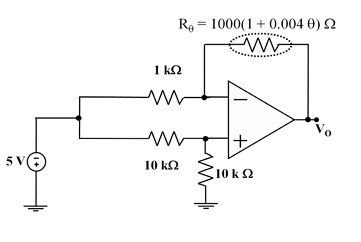
\includegraphics[width=0.7\columnwidth]{figs/z27.jpg}
\caption*{}
\label{fig:z27}
\end{figure}

\hfill{(GATE IN 2016)}

\item The photo diode in the figure below\figref{fig:z28} has an active sensing area of $10$ mm$^2$, a sensitivity of $0.5$ A/W and a dark current of $1$ $\mu$A. The i-to-v converter has a sensitivity of $100$ mV/$\mu$A. For an input light intensity of $4$ W/m$^2$, the output $V_o$ in volt is \rule{2cm}{0.4pt}.
\begin{figure}[H]
\centering
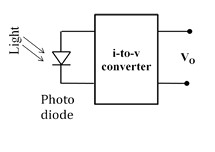
\includegraphics[width=0.5\columnwidth]{figs/z28.jpg}
\caption*{}
\label{fig:z28}
\end{figure}

\hfill{(GATE IN 2016)}

\item The velocity of flow of water \brak{\text{density $1000$ kg/m$^3$}} in a horizontal pipe is measured using the PITOT tube shown below.\figref{fig:z29} The fluid in the U-tube manometer is mercury with a density of $13534$ kg/m$^3$. Assume $g = 9.81$ m/s$^2$. If the height difference \brak{h} is measured as $94.1$ mm, the velocity of flow of water in m/s is \rule{2cm}{0.4pt}.
\begin{figure}[h!]
\centering
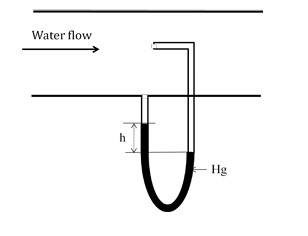
\includegraphics[width=0.6\columnwidth]{figs/z29.jpg}
\caption*{}
\label{fig:z29}
\end{figure}

\hfill{(GATE IN 2016)}

\item The bandgap in eV of a semiconductor material required to construct an LED that emits peak power at the wavelength of $620$ nm is \rule{2cm}{0.4pt}.

\brak{\text{Plank constant $h = 4.13567 \times 10^{-15}$ eV s and speed of light $c = 2.998 \times 10^8$ m/s}}.

\hfill{(GATE IN 2016)}

\item The signal $m\brak{t} = \frac{\sin\brak{100 \pi t}}{100 \pi t}$ is frequency modulated \brak{FM} with an FM modulator of frequency deviation constant of $30$ kHz/V. Using Carson's rule, the approximate bandwidth of the modulated wave in kilohertz is \rule{2cm}{0.4pt}.

\hfill{(GATE IN 2016)}

\item A signal $m\brak{t}$ varies from $-3.5$ V to $+3.5$ V with an average power of $3$ W. The signal is quantized using a midtread type quantizer and subsequently binary encoded. With the codeword of length 3, the signal to quantization noise ratio in dB is \rule{2cm}{0.4pt}.

\hfill{(GATE IN 2016)}

\end{enumerate}
\end{document}```